\documentclass[12pt,a4paper]{article}
\usepackage{caption}
\usepackage{float}
\usepackage[left=2cm, right=2cm, top=2cm, bottom=2cm]{geometry}
\usepackage{graphicx}
\usepackage{subcaption}
\usepackage{xeCJK}

\captionsetup[figure]{labelformat=empty}
\subcaptionsetup[figure]{labelformat=empty}
\setCJKmainfont{新細明體}

\title{
  Quartus II Lab2 \textemdash\ Sequential Circuits\\
  \large NTU Switching Circuit and Logic Design 2023
}
\author{B12902110 呂承諺}
\date{}

\begin{document}
  \maketitle
  \section{Lab2\_1}
  \subsection{SD: Sequence Detector}
  \begin{figure}[H]
    \centering
    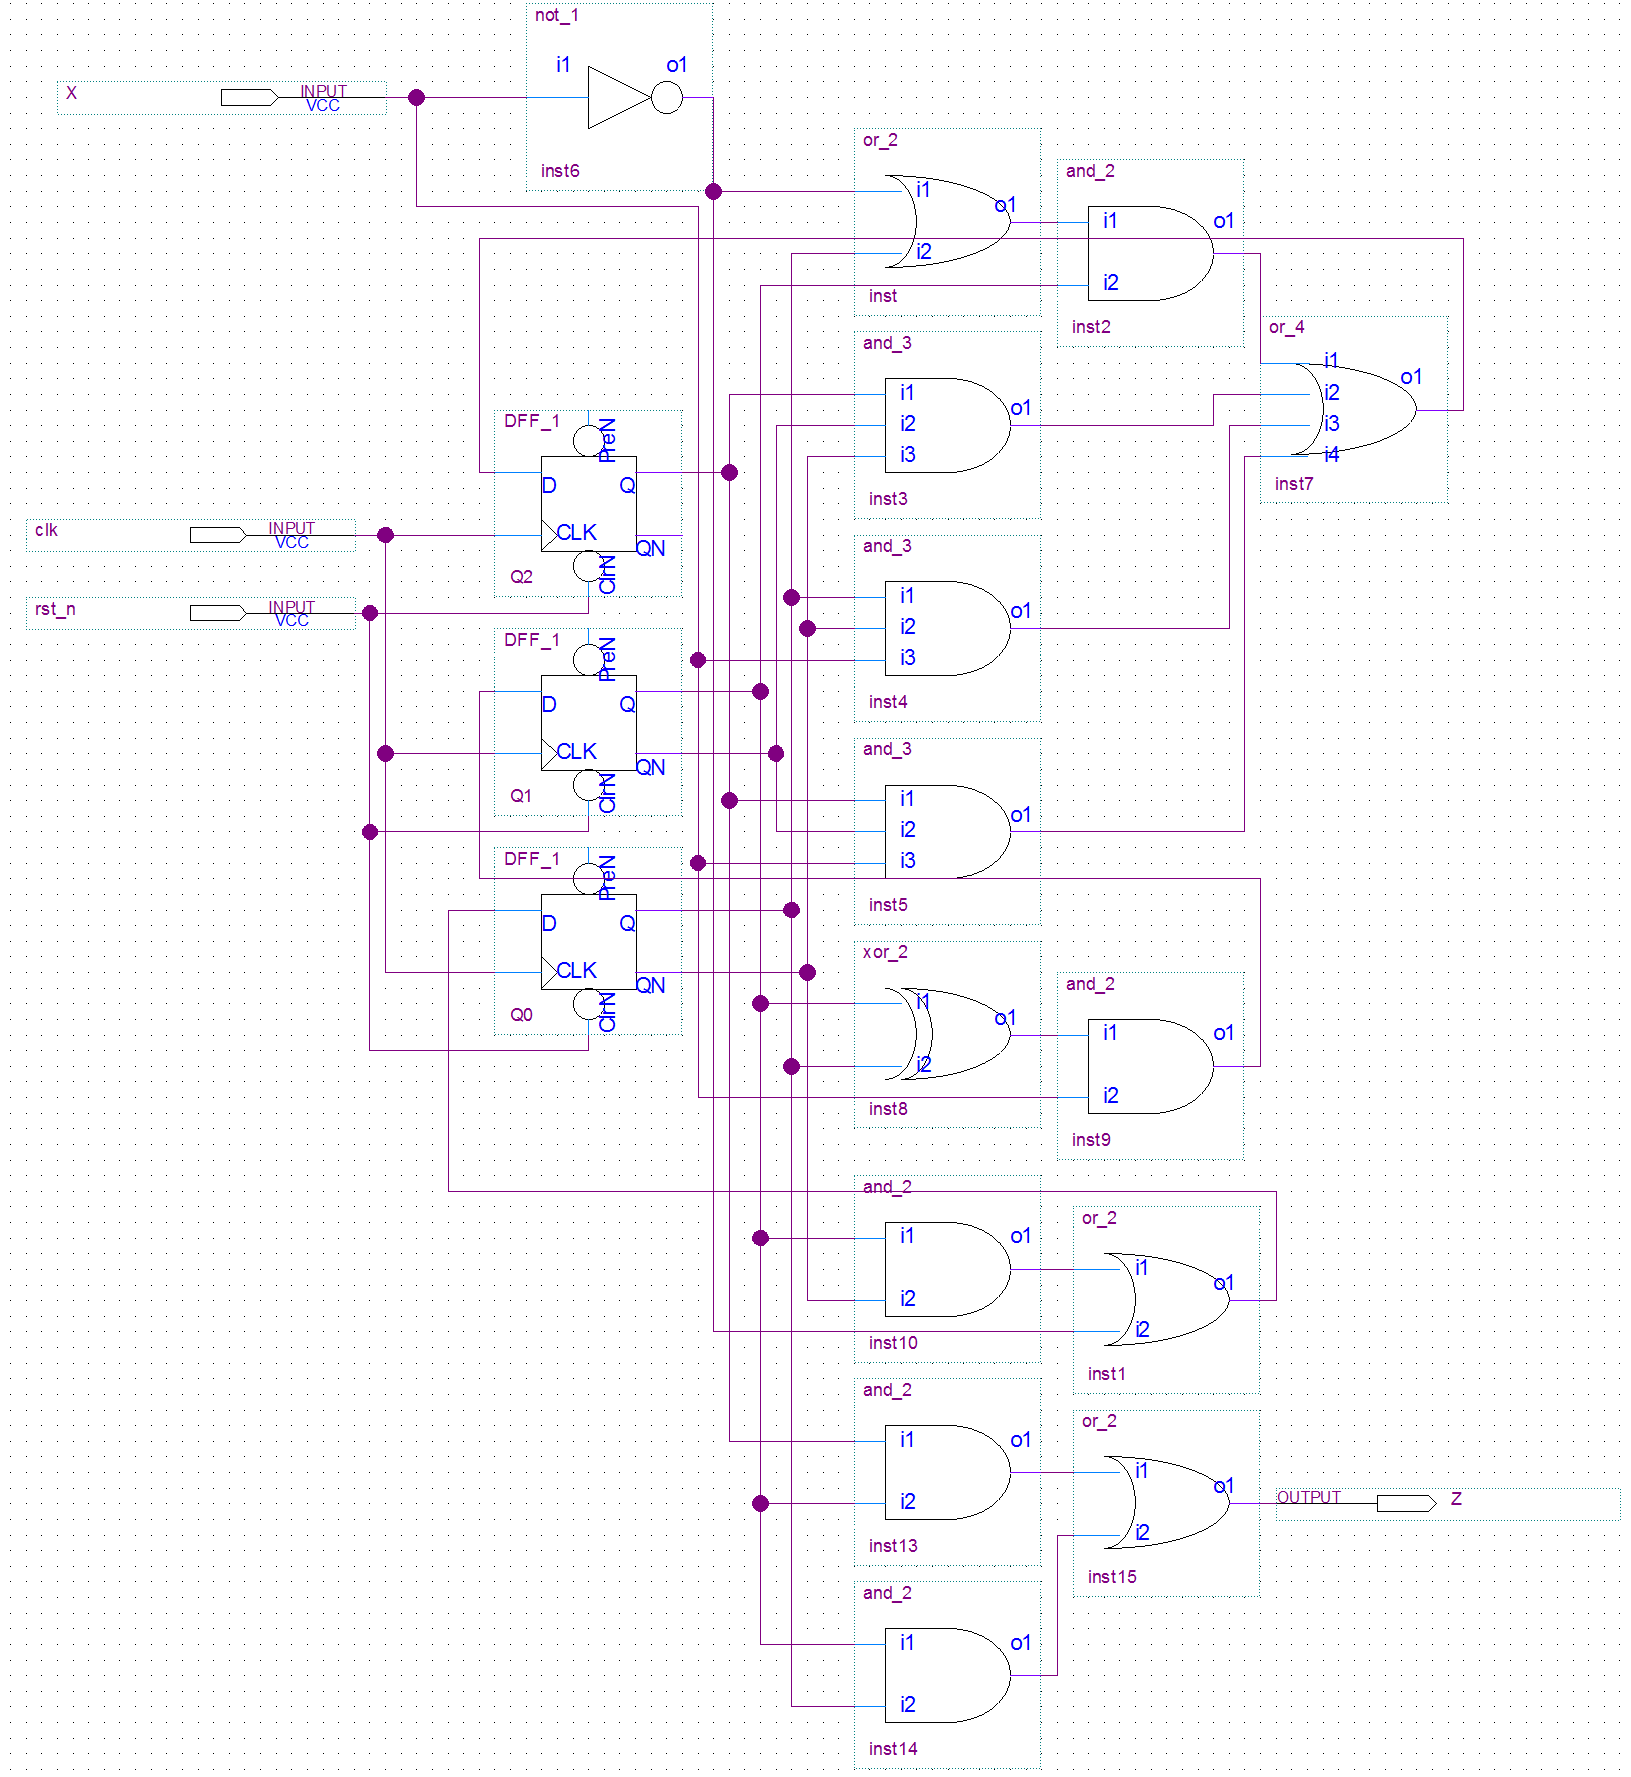
\includegraphics[width=0.93\linewidth]{Lab2_1/SD_bdf.png}
    \caption{SD.bdf}
  \end{figure}
  \begin{figure}[H]
    \centering
    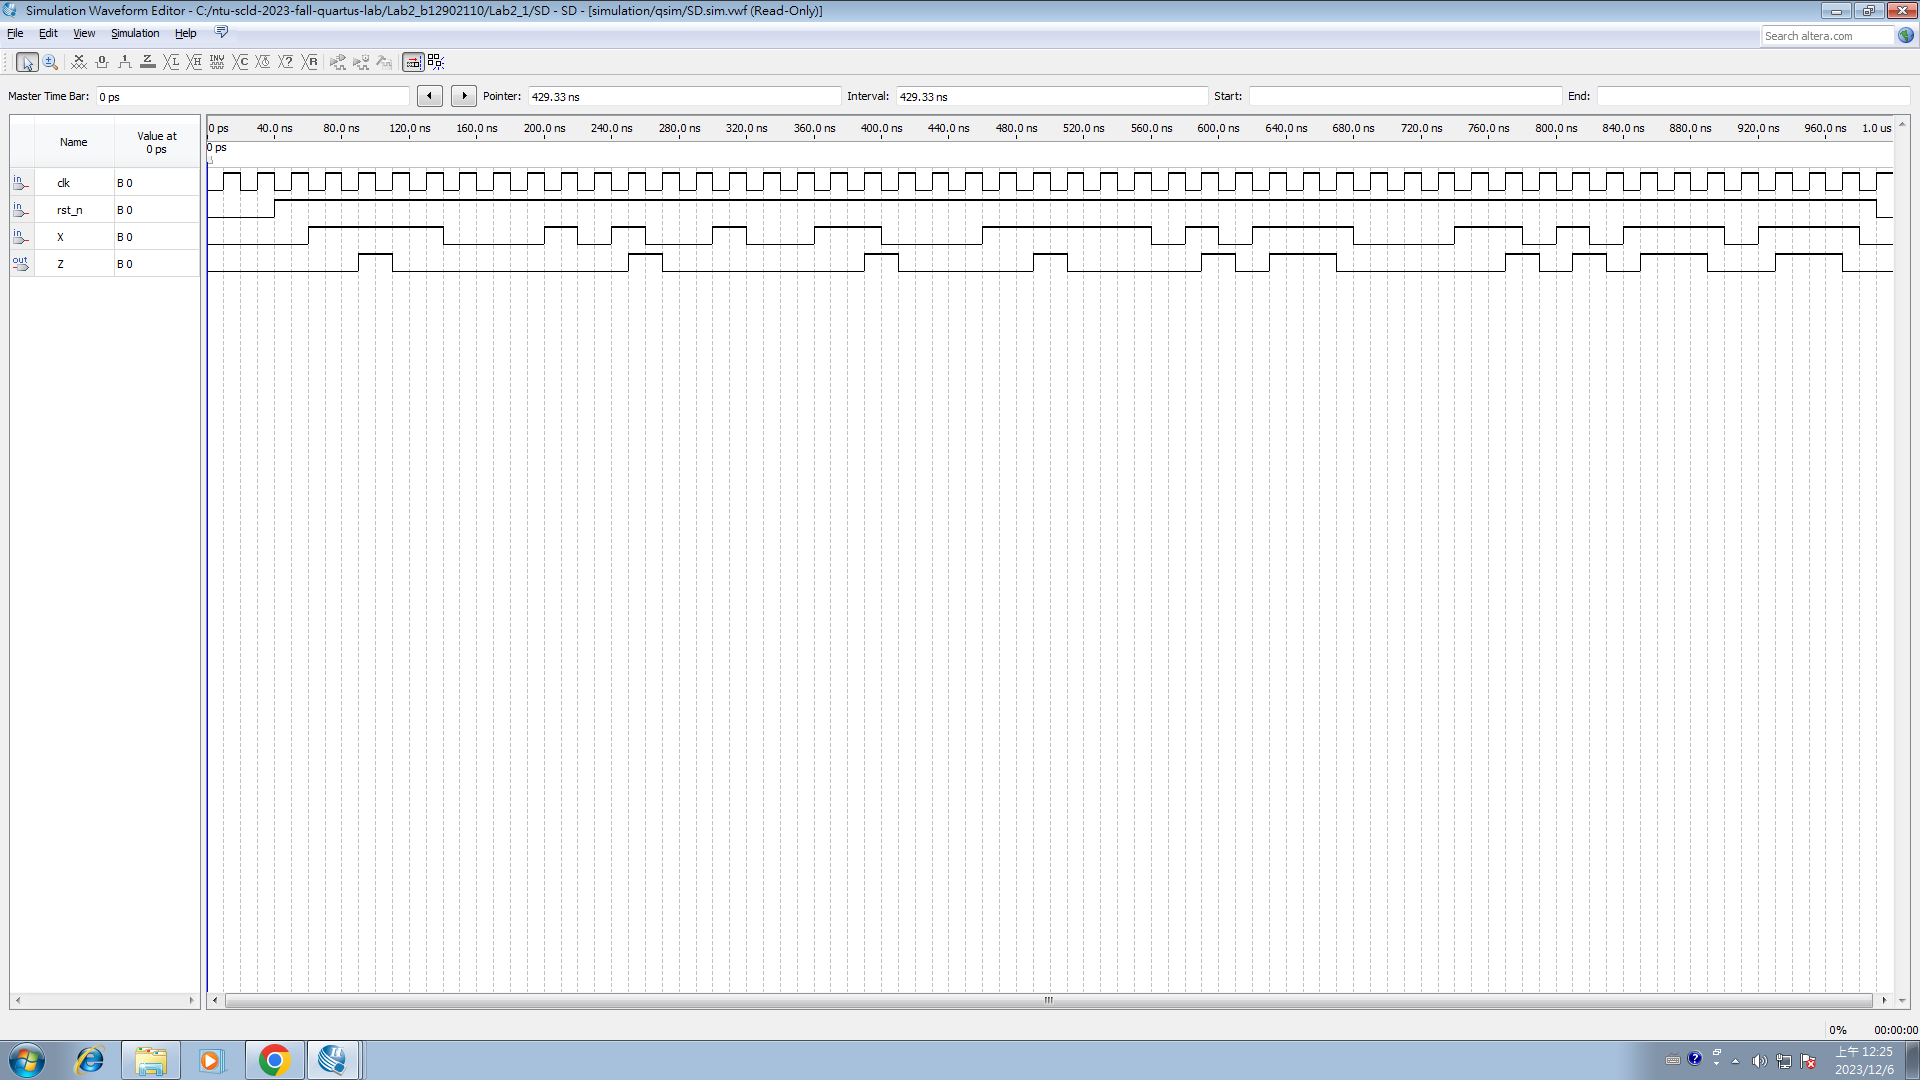
\includegraphics[width=\linewidth]{Lab2_1/SD_simulation.png}
    \caption{SD simulation result}
  \end{figure}

  \section{Lab2\_2}
  \subsection{FA: 1-bit Full Adder}
  \begin{figure}[H]
    \centering
    \begin{subcaptionblock}{0.15\linewidth}
      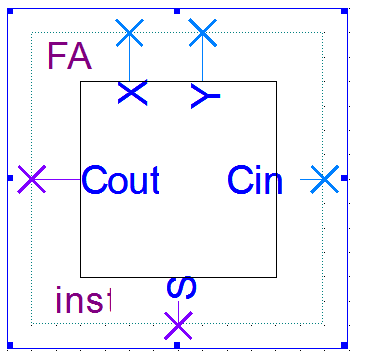
\includegraphics[width=\linewidth]{Lab2_2/FA_bsf.png}
      \caption{FA.bsf}
    \end{subcaptionblock}
    \begin{subcaptionblock}{0.84\linewidth}
      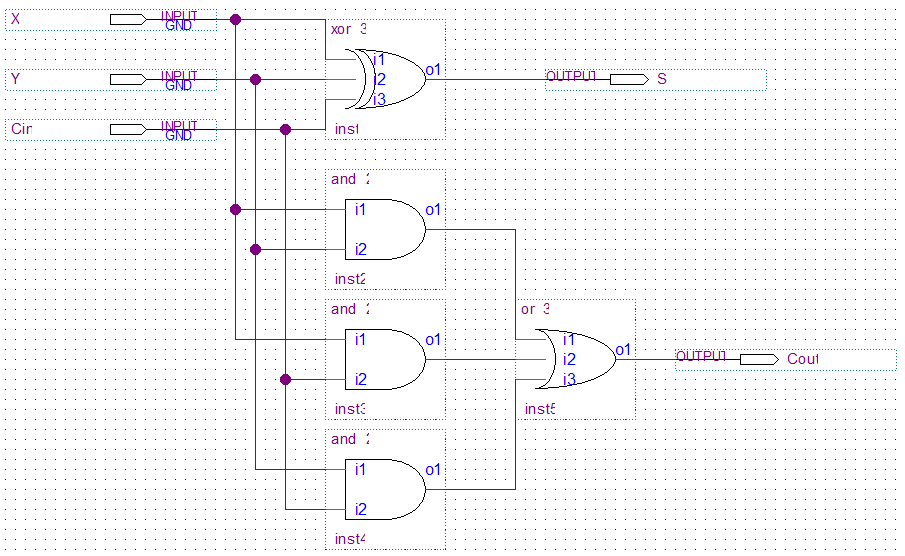
\includegraphics[width=\linewidth]{Lab2_2/FA_bdf.png}
      \caption{FA.bdf}
    \end{subcaptionblock}
  \end{figure}

  \subsection{FA4: 4-bit Adder}
  \begin{figure}[H]
    \centering
    \begin{subcaptionblock}{0.15\linewidth}
      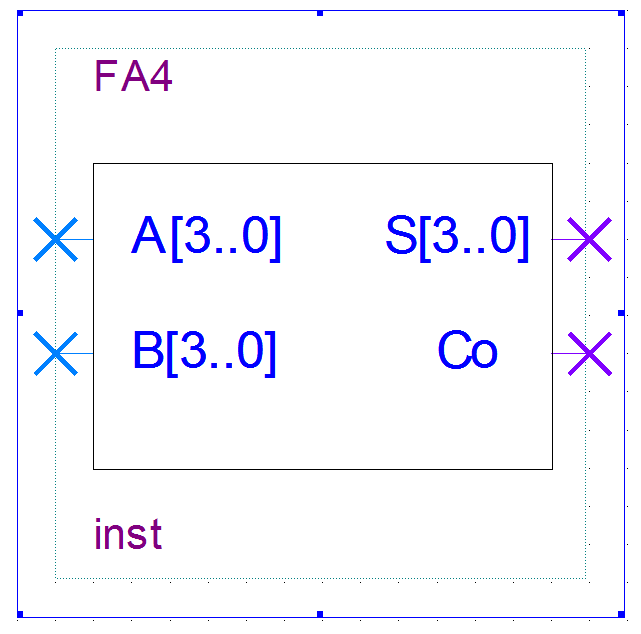
\includegraphics[width=\linewidth]{Lab2_2/FA4_bsf.png}
      \caption{FA4.bsf}
    \end{subcaptionblock}
    \begin{subcaptionblock}{0.84\linewidth}
      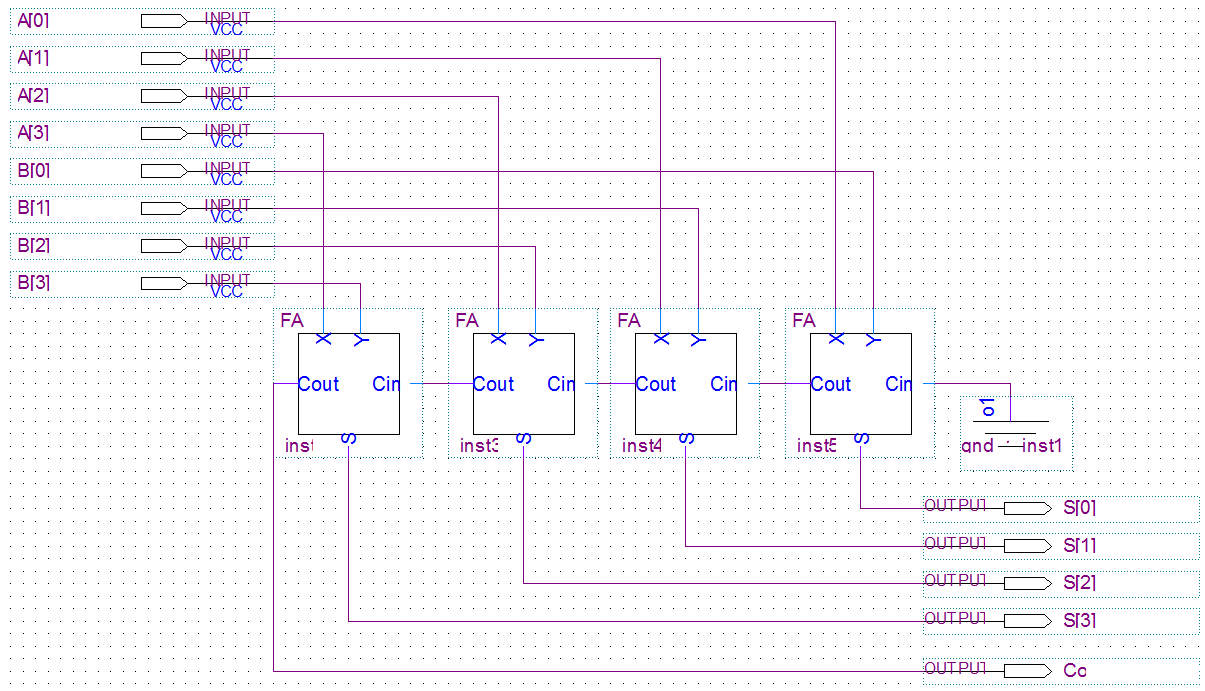
\includegraphics[width=\linewidth]{Lab2_2/FA4_bdf.png}
      \caption{FA4.bdf}
    \end{subcaptionblock}
  \end{figure}

  \subsection{MUX1: 1-bit 2-to-1 Multiplexer}
  \begin{figure}[H]
    \centering
    \begin{subcaptionblock}{0.15\linewidth}
      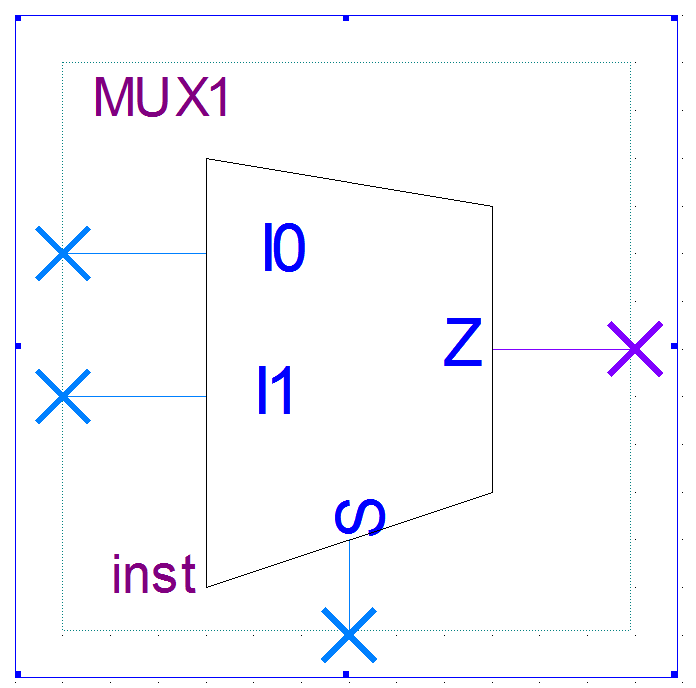
\includegraphics[width=\linewidth]{Lab2_2/MUX1_bsf.png}
      \caption{MUX1.bsf}
    \end{subcaptionblock}
    \begin{subcaptionblock}{0.84\linewidth}
      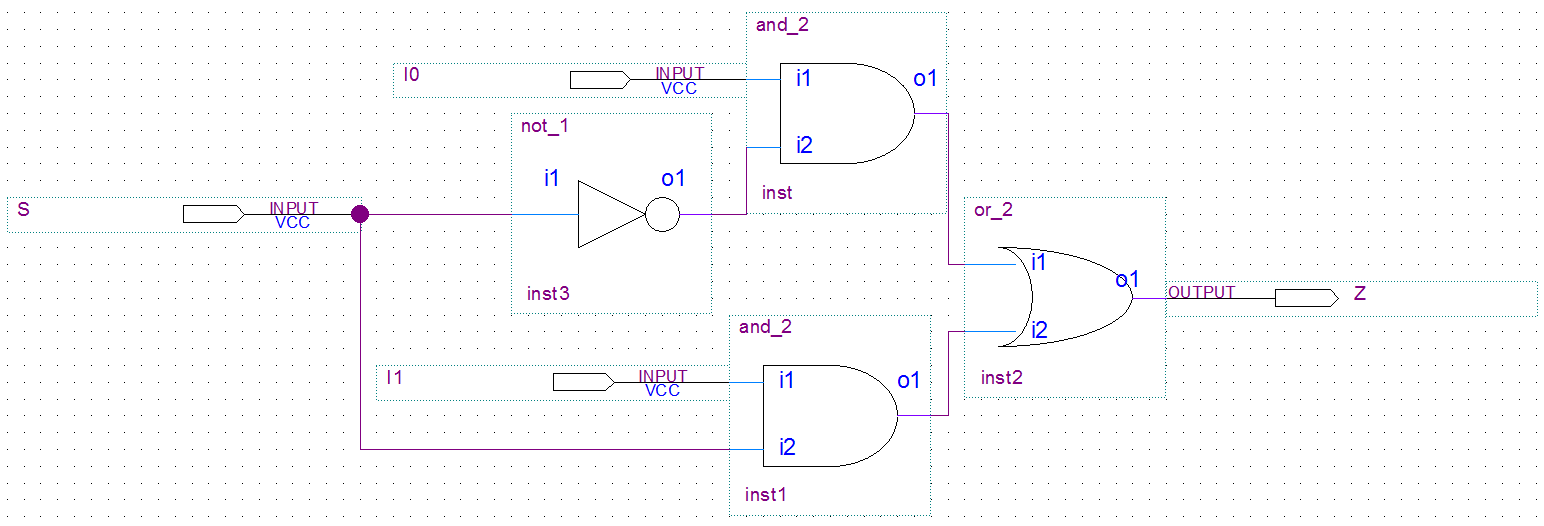
\includegraphics[width=\linewidth]{Lab2_2/MUX1_bdf.png}
      \caption{MUX1.bdf}
    \end{subcaptionblock}
  \end{figure}

  \subsection{MUX4: 4-bit 2-to-1 Multiplexer}
  \begin{figure}[H]
    \centering
    \begin{subcaptionblock}{0.19\linewidth}
      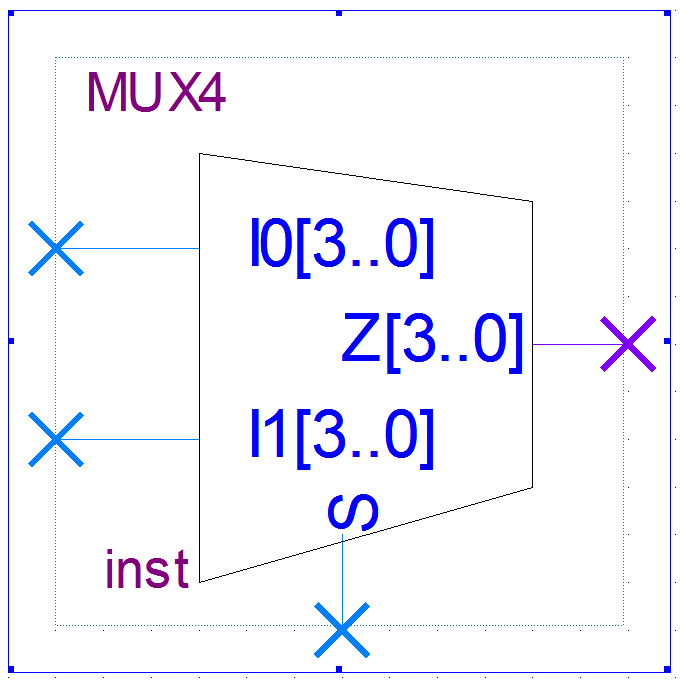
\includegraphics[width=\linewidth]{Lab2_2/MUX4_bsf.png}
      \caption{MUX4.bsf}
    \end{subcaptionblock}
    \begin{subcaptionblock}{0.8\linewidth}
      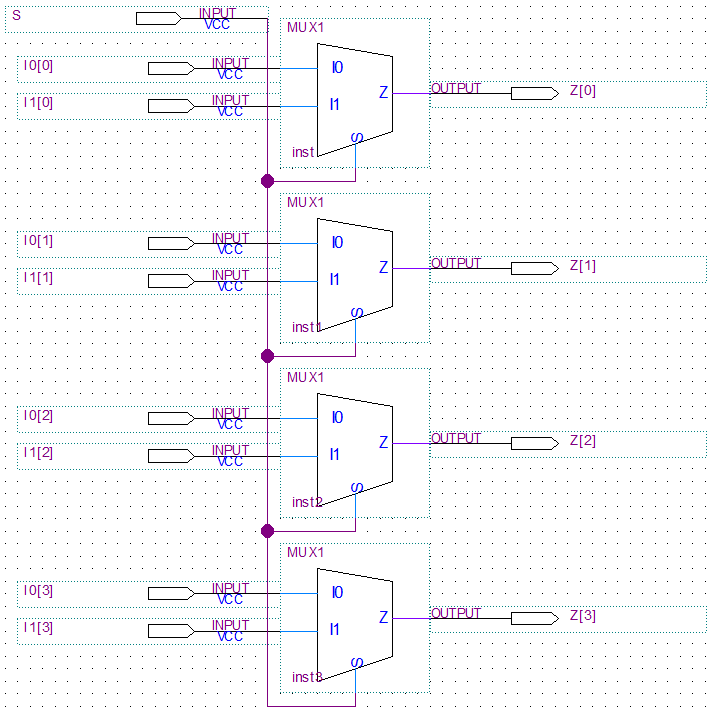
\includegraphics[width=\linewidth]{Lab2_2/MUX4_bdf.png}
      \caption{MUX4.bdf}
    \end{subcaptionblock}
  \end{figure}

  \subsection{Register: 4-bit Register}
  \begin{figure}[H]
    \centering
    \begin{subcaptionblock}{0.19\linewidth}
      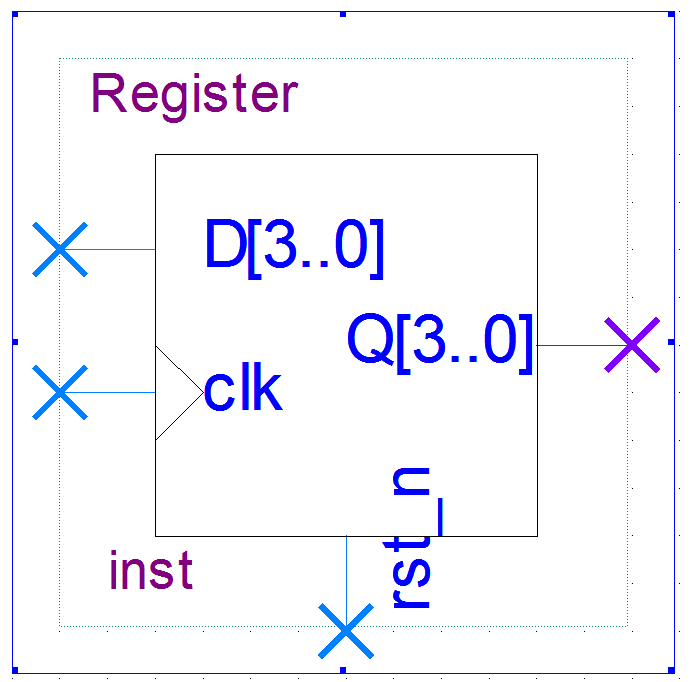
\includegraphics[width=\linewidth]{Lab2_2/Register_bsf.png}
      \caption{Register.bsf}
    \end{subcaptionblock}
    \begin{subcaptionblock}{0.8\linewidth}
      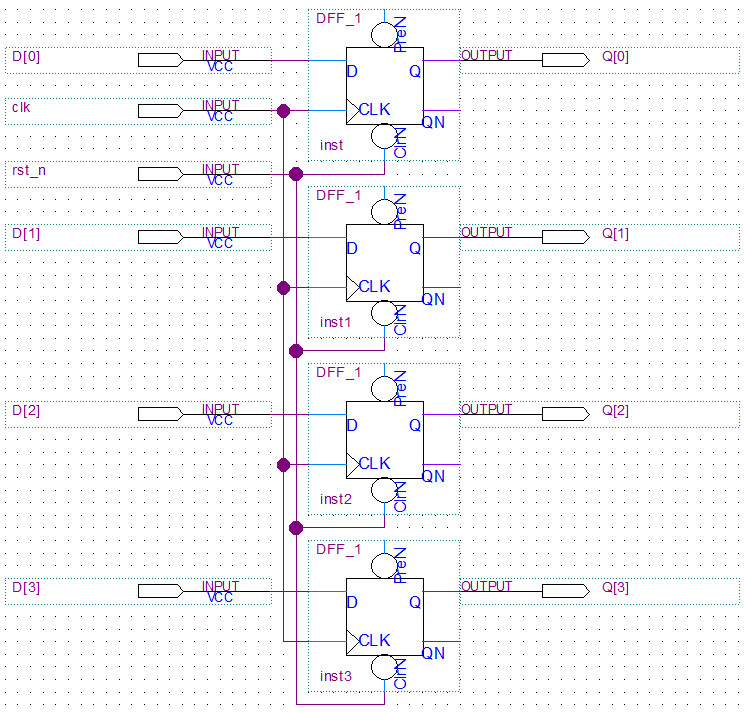
\includegraphics[width=\linewidth]{Lab2_2/Register_bdf.png}
      \caption{Register.bdf}
    \end{subcaptionblock}
  \end{figure}

  \subsection{Controller: Finite-state Machine}
  \begin{figure}[H]
    \centering
    \begin{subcaptionblock}{0.19\linewidth}
      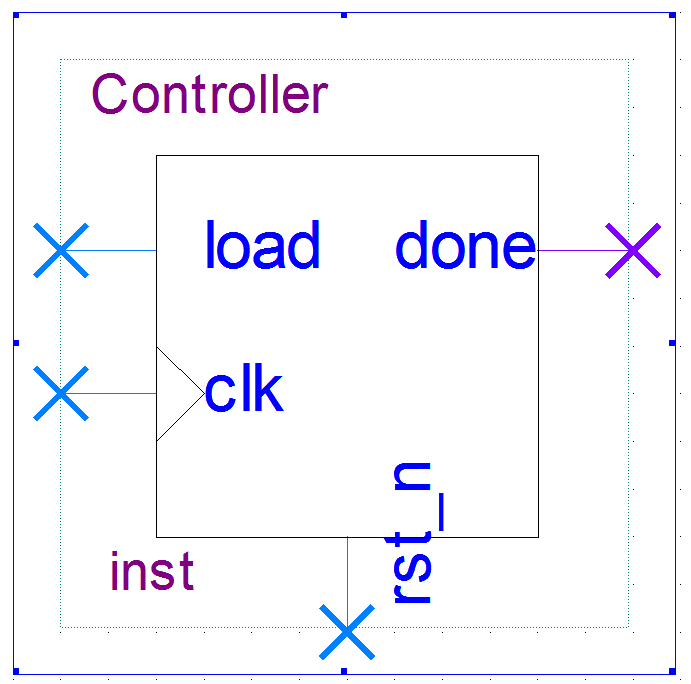
\includegraphics[width=\linewidth]{Lab2_2/Controller_bsf.png}
      \caption{Controller.bsf}
    \end{subcaptionblock}
    \begin{subcaptionblock}{0.8\linewidth}
      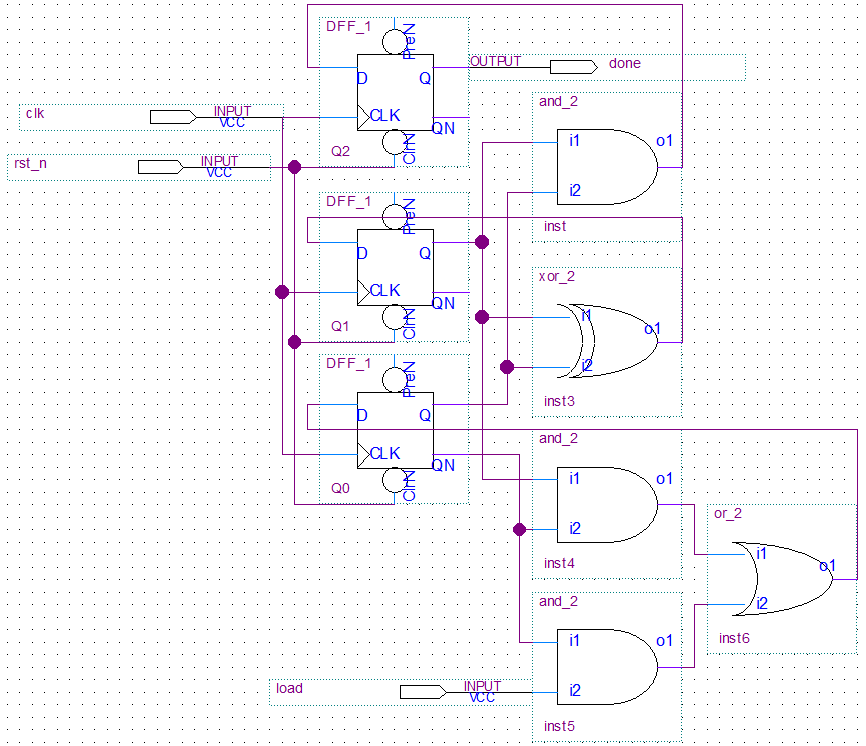
\includegraphics[width=\linewidth]{Lab2_2/Controller_bdf.png}
      \caption{Controller.bdf}
    \end{subcaptionblock}
  \end{figure}

  \subsection{AC4: 4-bit Accmulator}
  \begin{figure}[H]
    \centering
    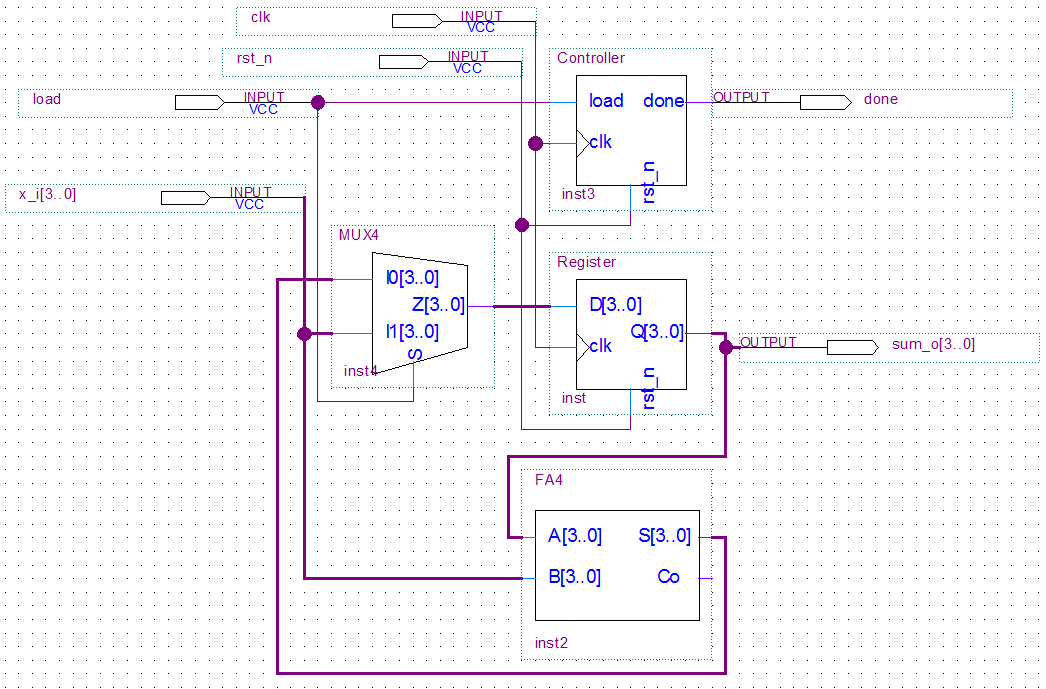
\includegraphics[width=\linewidth]{Lab2_2/AC4_bdf.png}
    \caption{AC4.bdf}
  \end{figure}
  \begin{figure}[H]
    \centering
    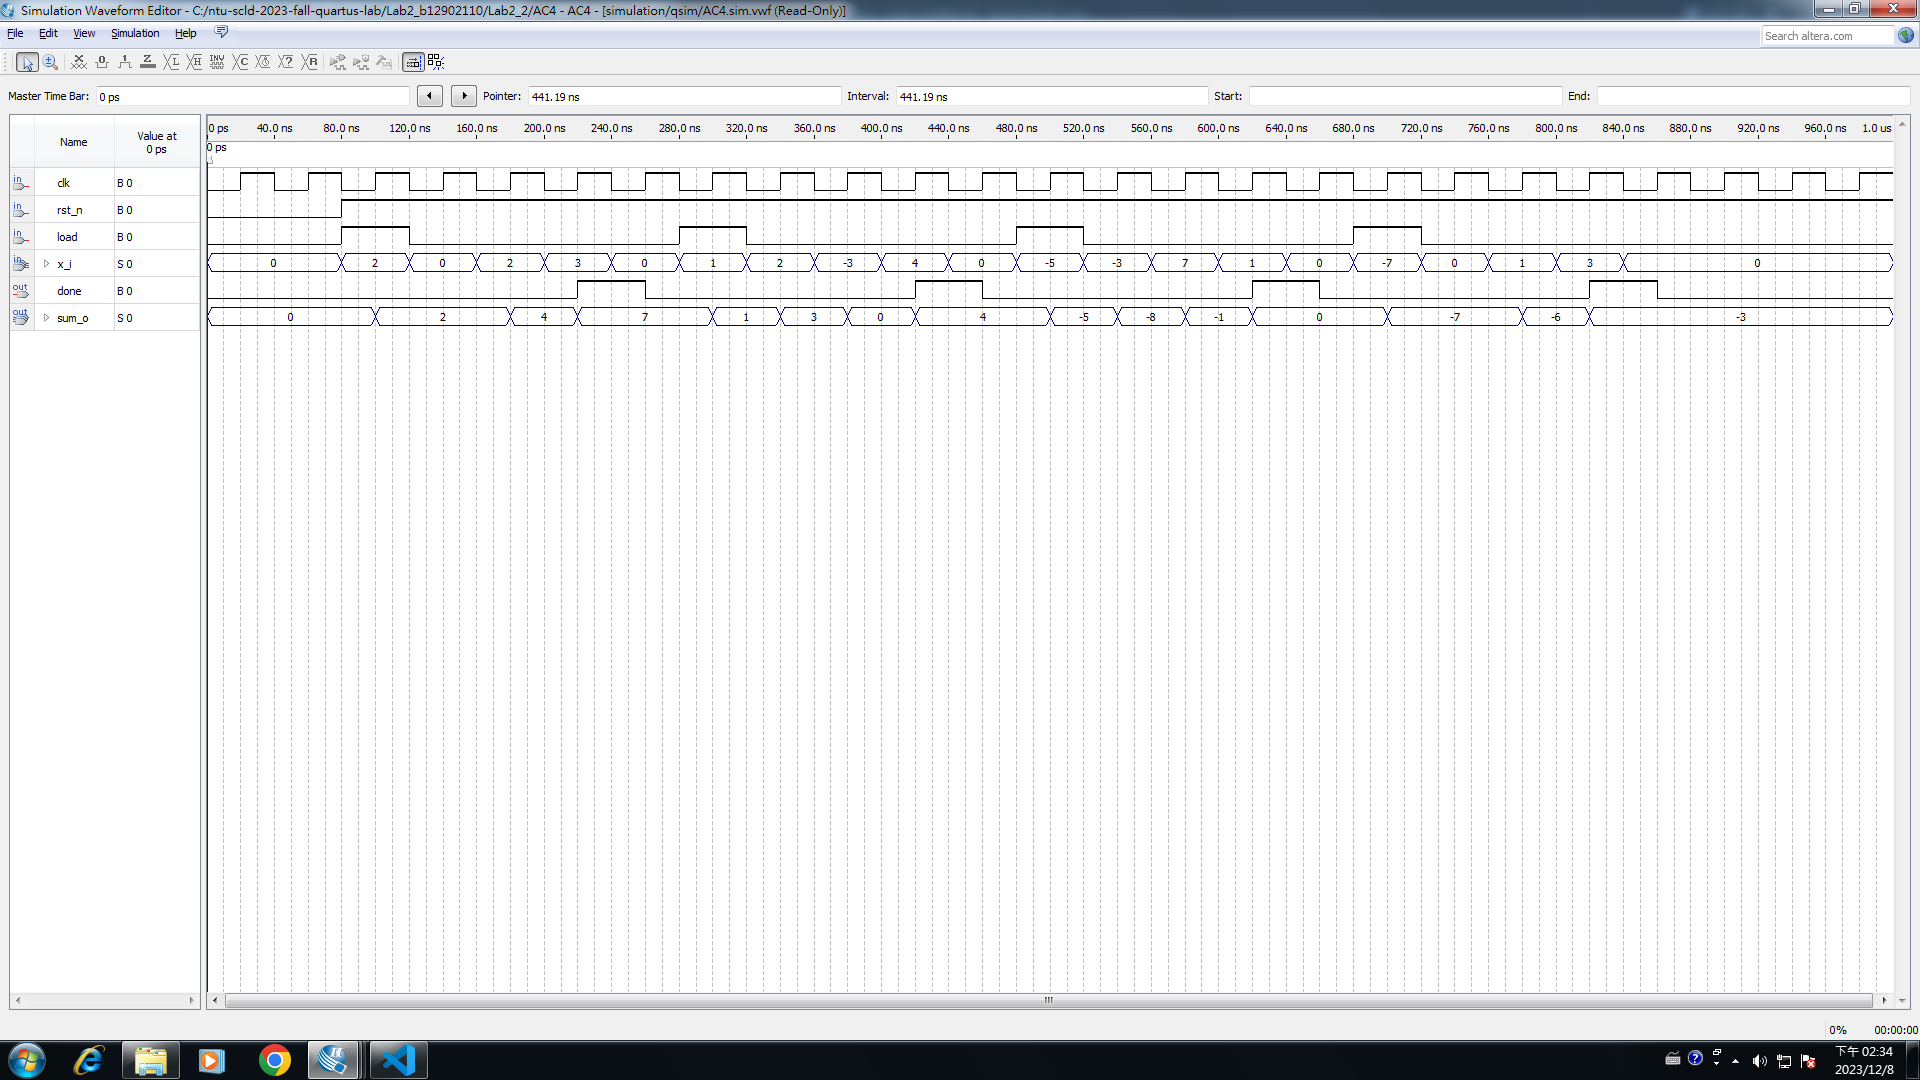
\includegraphics[width=\linewidth]{Lab2_2/AC4_simulation.png}
    \caption{AC4 simulation result}
  \end{figure}

  \section{Lab2\_3}
  \subsection{FA: 1-bit Full Adder}
  \begin{figure}[H]
    \centering
    \begin{subcaptionblock}{0.15\linewidth}
      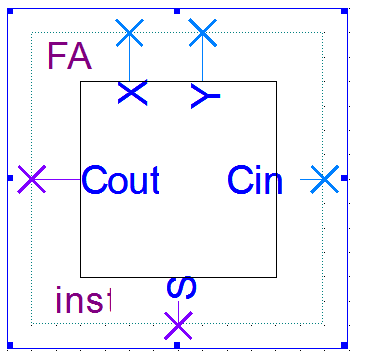
\includegraphics[width=\linewidth]{Lab2_2/FA_bsf.png}
      \caption{FA.bsf}
    \end{subcaptionblock}
    \begin{subcaptionblock}{0.84\linewidth}
      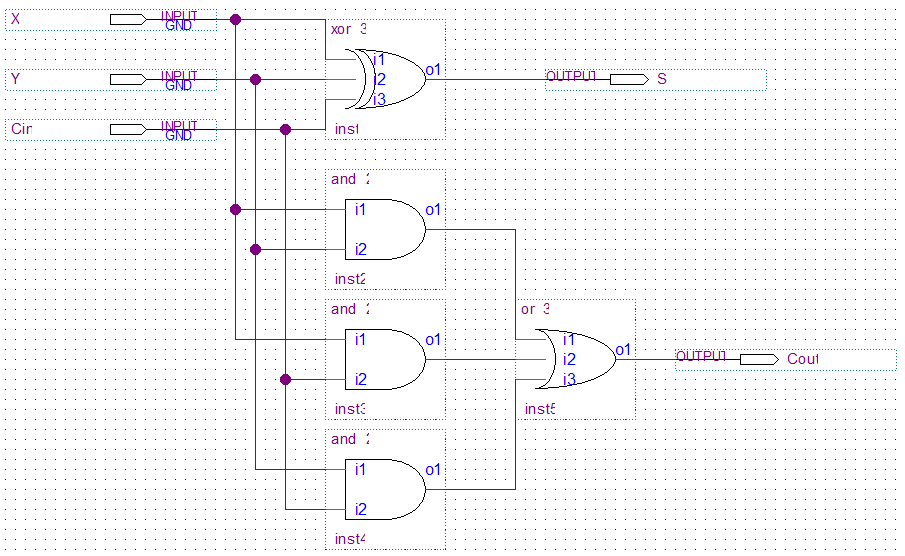
\includegraphics[width=\linewidth]{Lab2_2/FA_bdf.png}
      \caption{FA.bdf}
    \end{subcaptionblock}
  \end{figure}

  \subsection{FA4: 4-bit Adder}
  \begin{figure}[H]
    \centering
    \begin{subcaptionblock}{0.15\linewidth}
      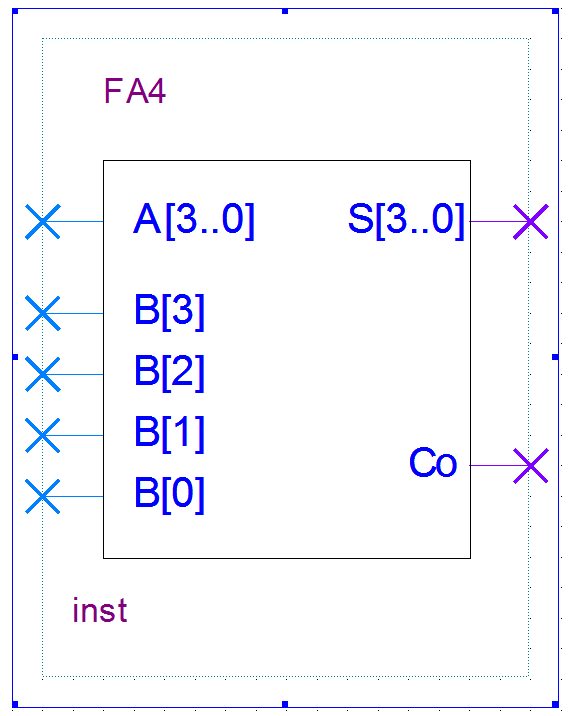
\includegraphics[width=\linewidth]{Lab2_3/FA4_bsf.png}
      \caption{FA4.bsf}
    \end{subcaptionblock}
    \begin{subcaptionblock}{0.84\linewidth}
      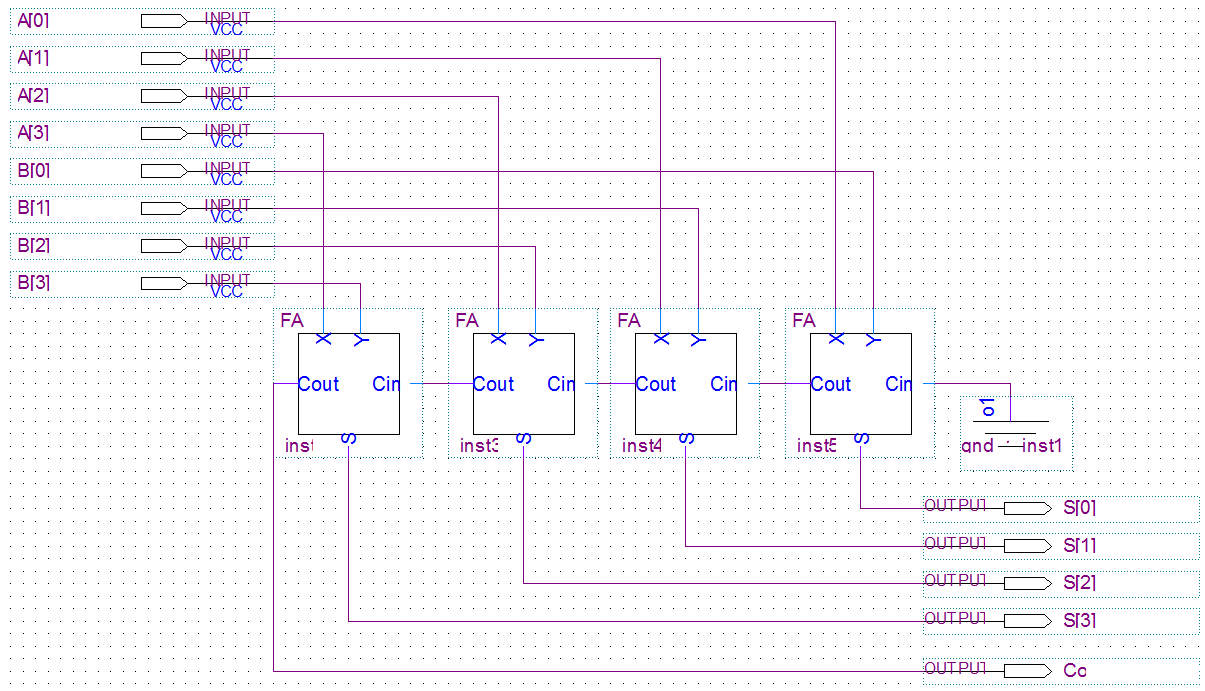
\includegraphics[width=\linewidth]{Lab2_2/FA4_bdf.png}
      \caption{FA4.bdf}
    \end{subcaptionblock}
  \end{figure}

  \subsection{SD: Sequence Detector}
  \begin{figure}[H]
    \centering
    \begin{subcaptionblock}{0.15\linewidth}
      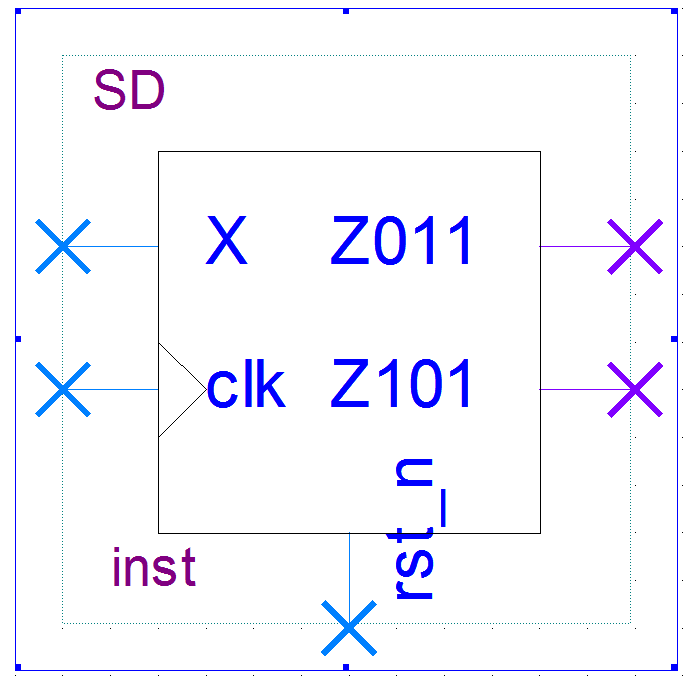
\includegraphics[width=\linewidth]{Lab2_3/SD_bsf.png}
      \caption{SD.bsf}
    \end{subcaptionblock}
    \begin{subcaptionblock}{0.84\linewidth}
      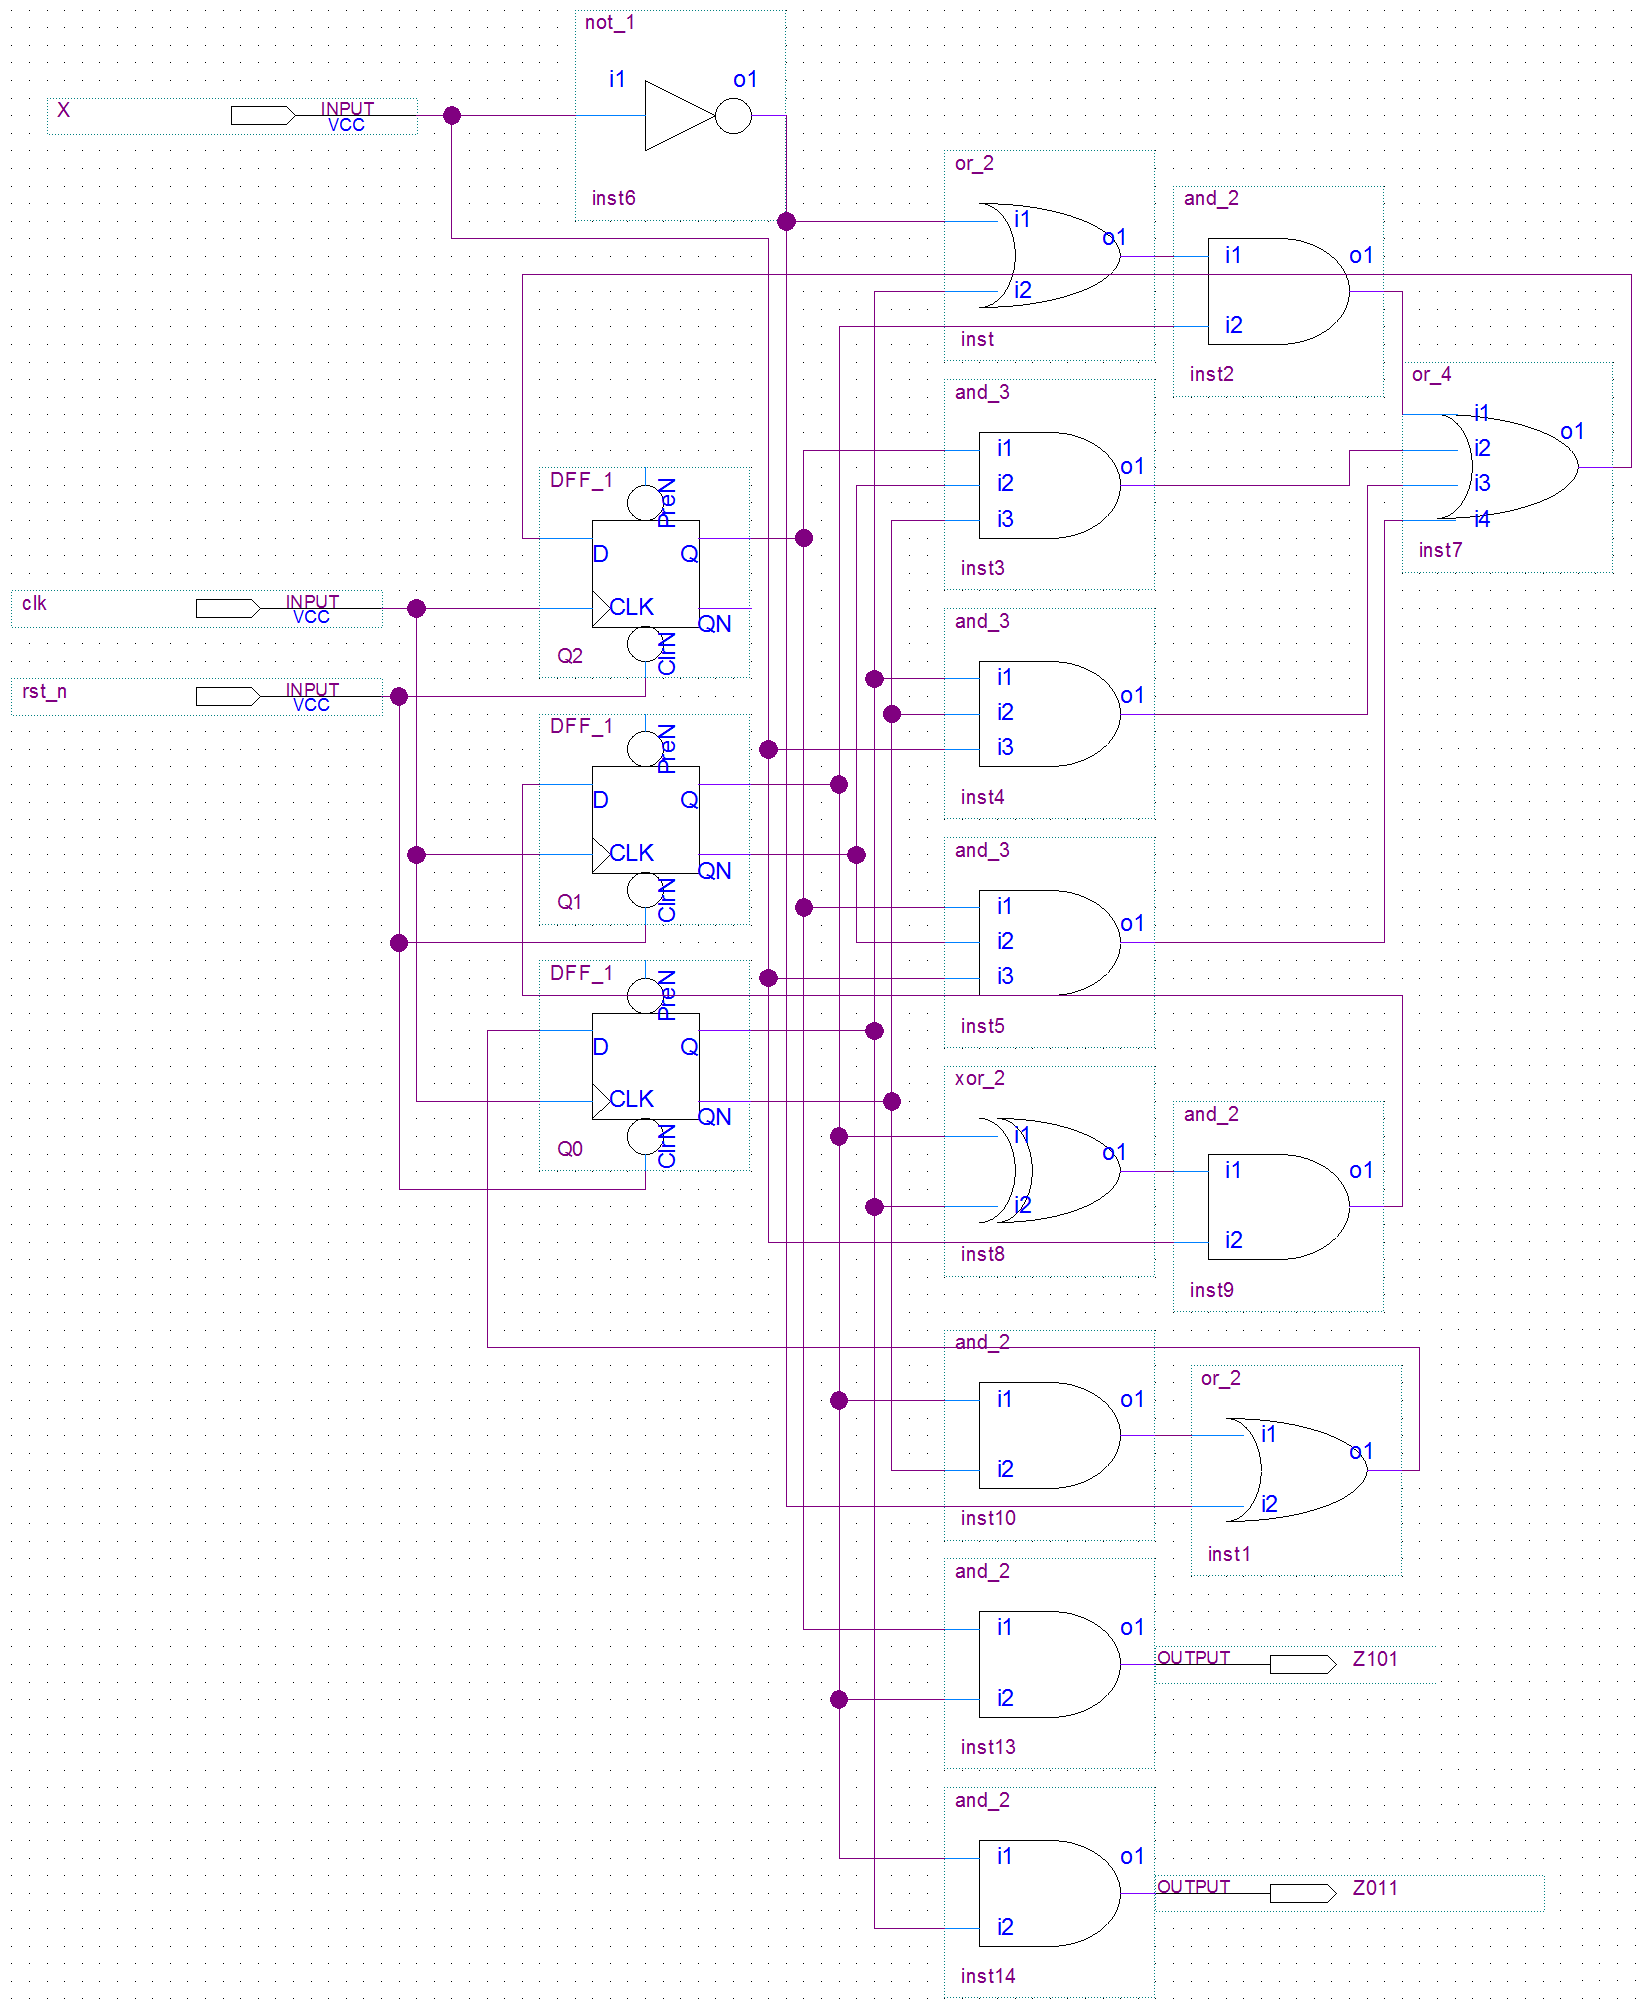
\includegraphics[width=\linewidth]{Lab2_3/SD_bdf.png}
      \caption{SD.bdf}
    \end{subcaptionblock}
  \end{figure}

  \subsection{Register: 4-bit Register}
  \begin{figure}[H]
    \centering
    \begin{subcaptionblock}{0.19\linewidth}
      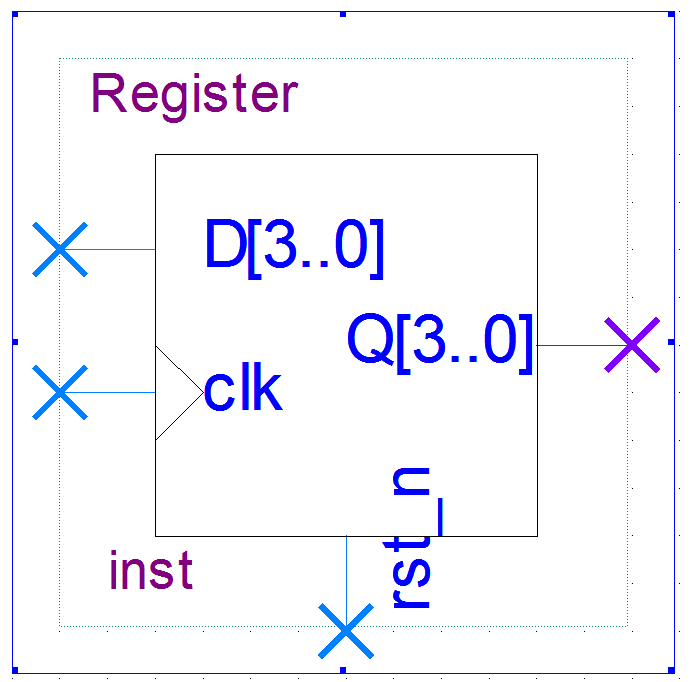
\includegraphics[width=\linewidth]{Lab2_2/Register_bsf.png}
      \caption{Register.bsf}
    \end{subcaptionblock}
    \begin{subcaptionblock}{0.8\linewidth}
      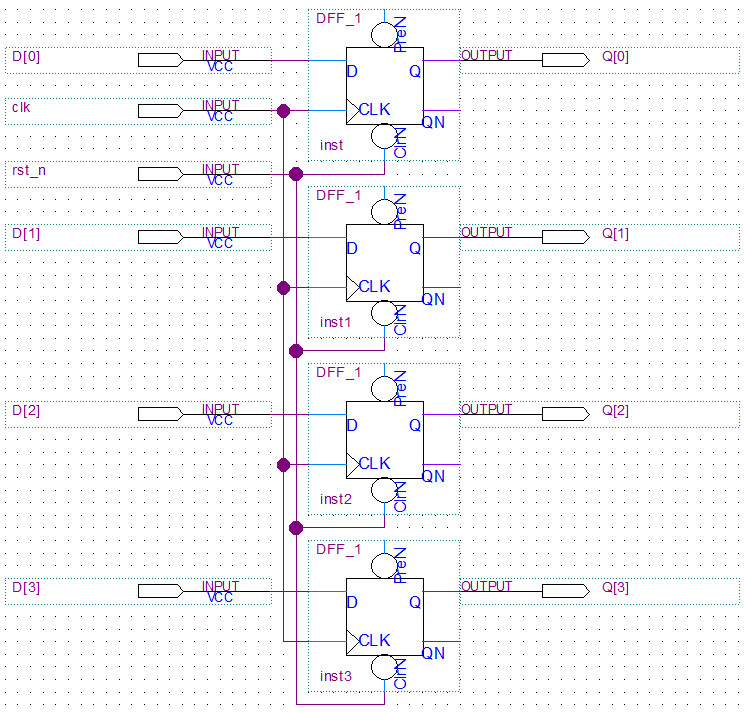
\includegraphics[width=\linewidth]{Lab2_2/Register_bdf.png}
      \caption{Register.bdf}
    \end{subcaptionblock}
  \end{figure}

  \subsection{Controller: Finite-state Machine}
  \begin{figure}[H]
    \centering
    \begin{subcaptionblock}{0.19\linewidth}
      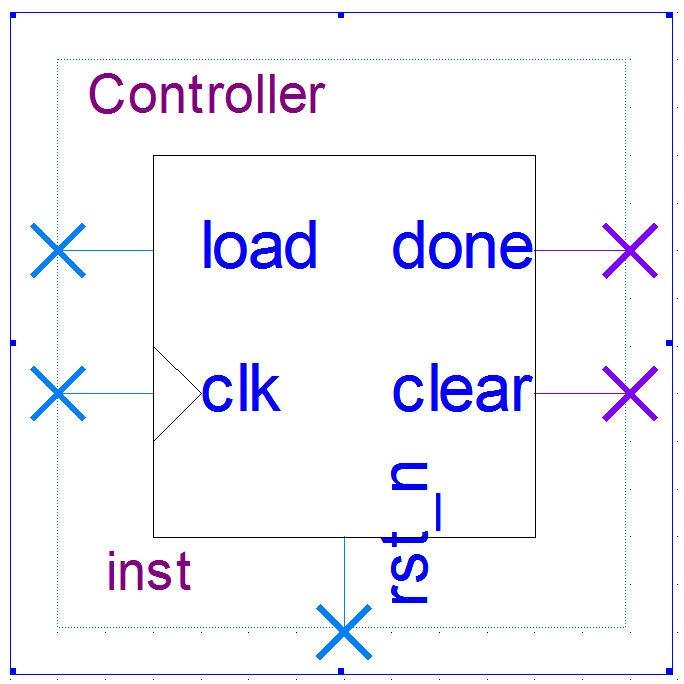
\includegraphics[width=\linewidth]{Lab2_3/Controller_bsf.png}
      \caption{Controller.bsf}
    \end{subcaptionblock}
    \begin{subcaptionblock}{0.8\linewidth}
      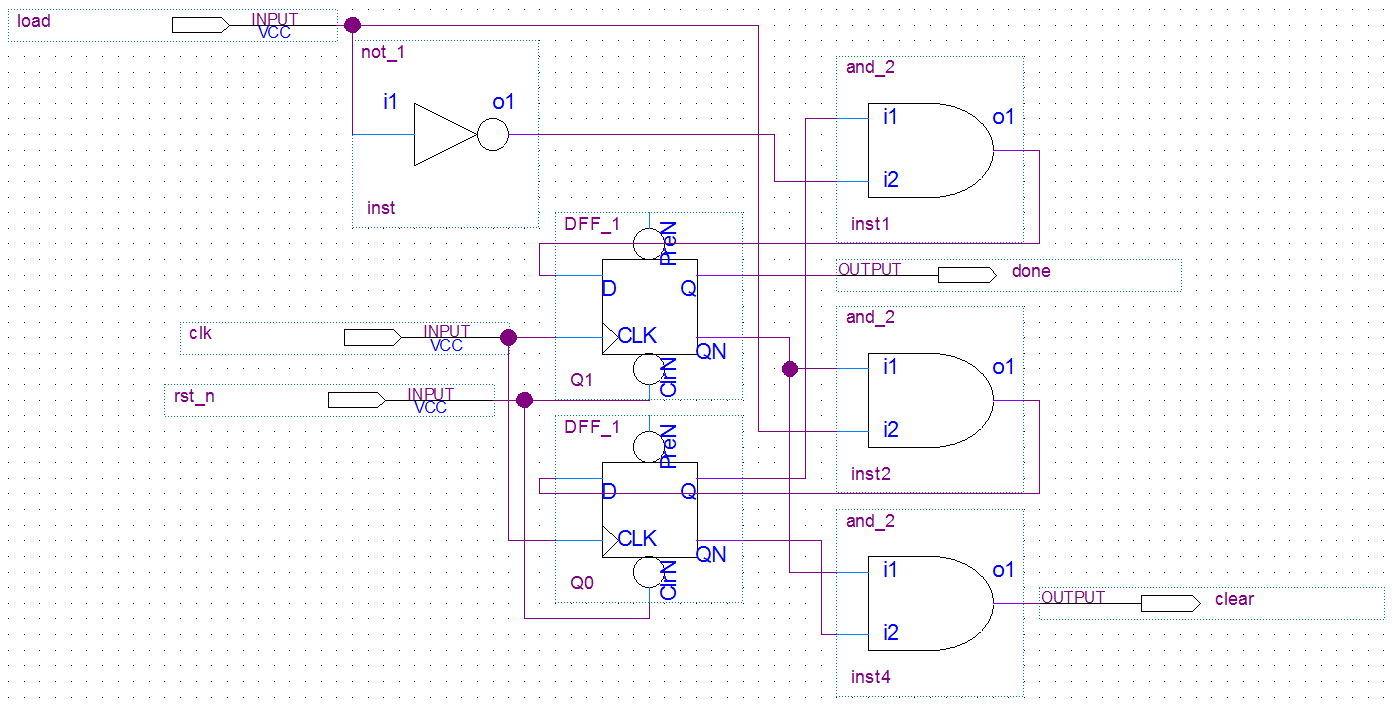
\includegraphics[width=\linewidth]{Lab2_3/Controller_bdf.png}
      \caption{Controller.bdf}
    \end{subcaptionblock}
  \end{figure}

  \subsection{WSC: Weighted Sequence Counter}
  \begin{figure}[H]
    \centering
    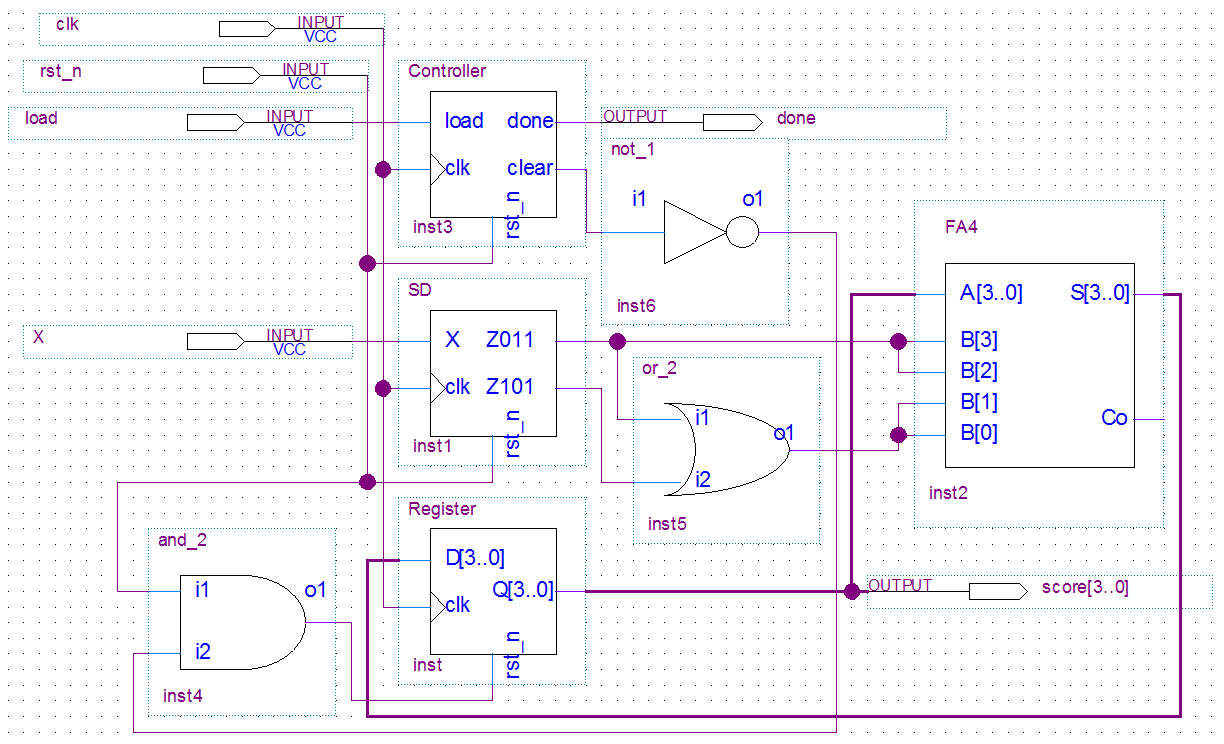
\includegraphics[width=\linewidth]{Lab2_3/WSC_bdf.png}
    \caption{WSC.bdf}
  \end{figure}
  \begin{figure}[H]
    \centering
    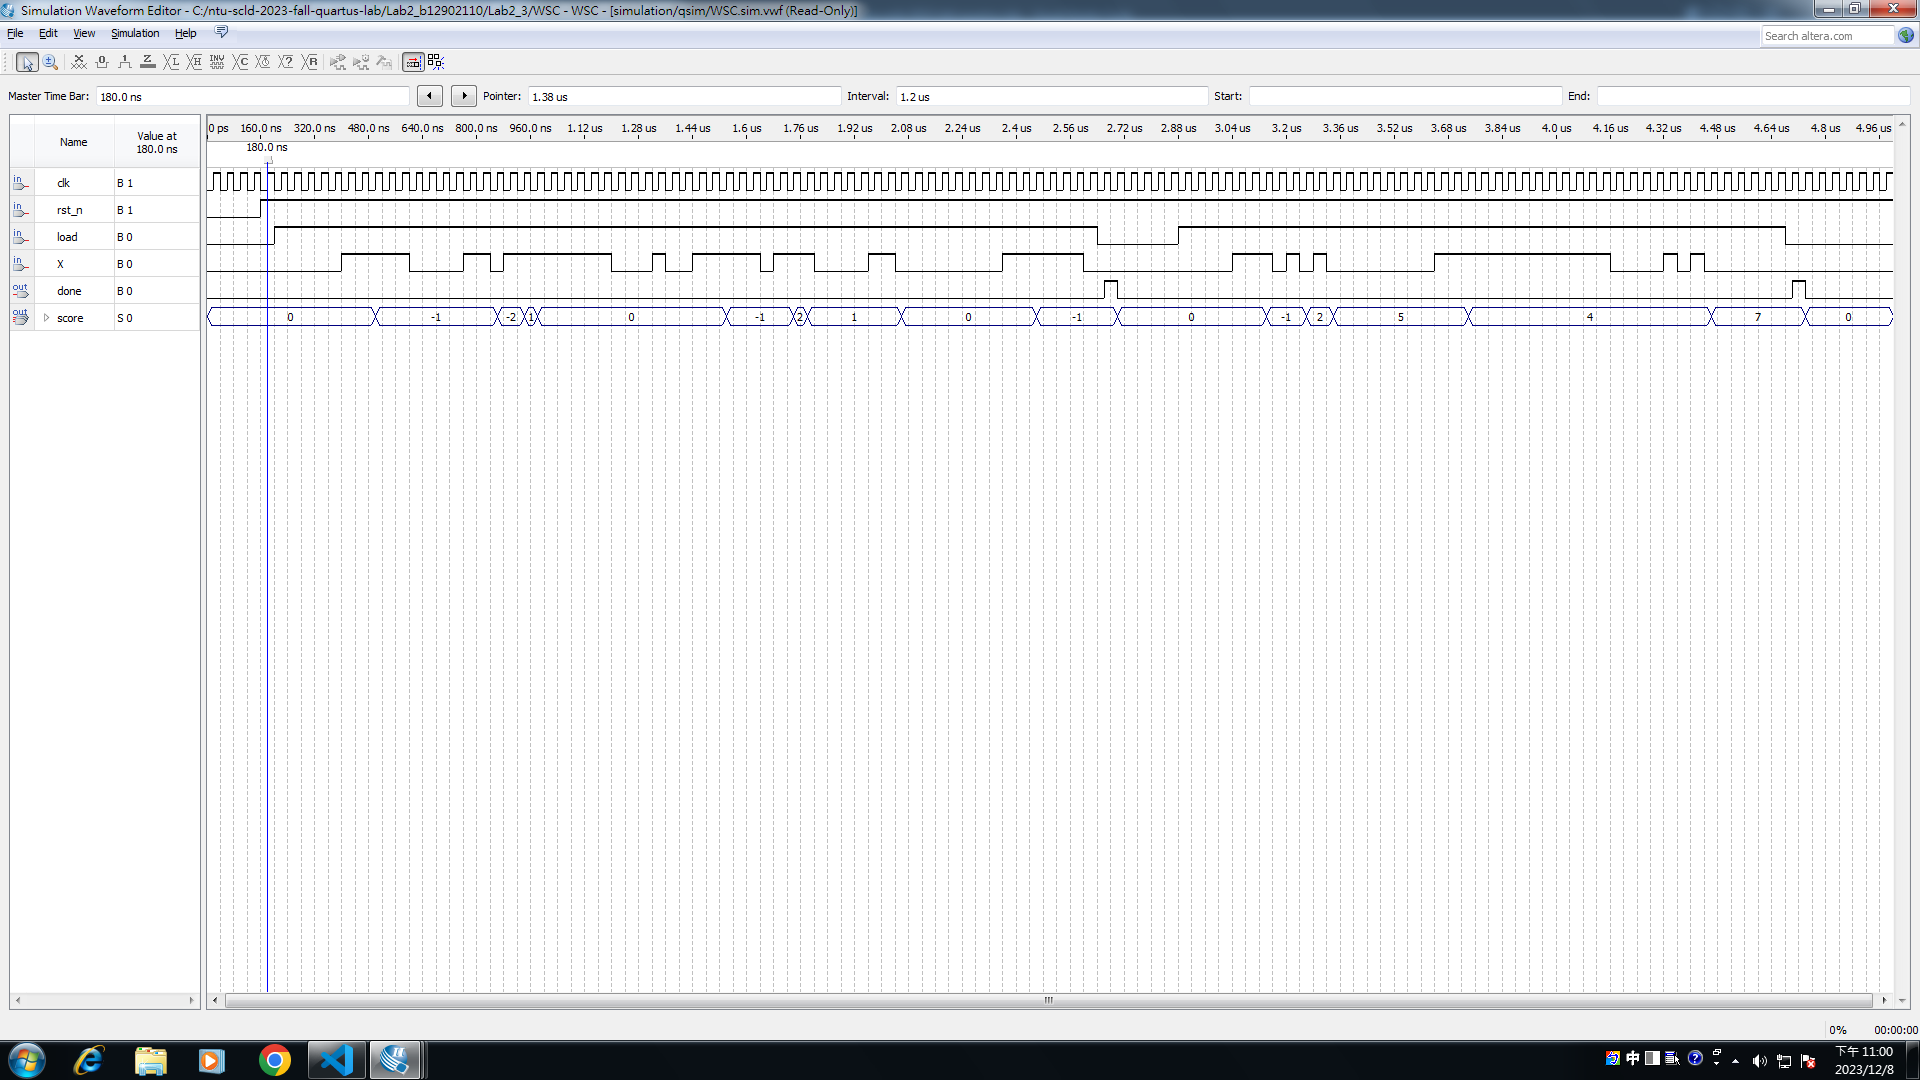
\includegraphics[width=\linewidth]{Lab2_3/WSC_simulation.png}
    \caption{WSC simulation result}
  \end{figure}
\end{document}
